\documentclass{standalone}
\usepackage{tikz}
\usepackage{amsmath}
\usetikzlibrary{arrows.meta, angles, quotes, calc}

\begin{document}
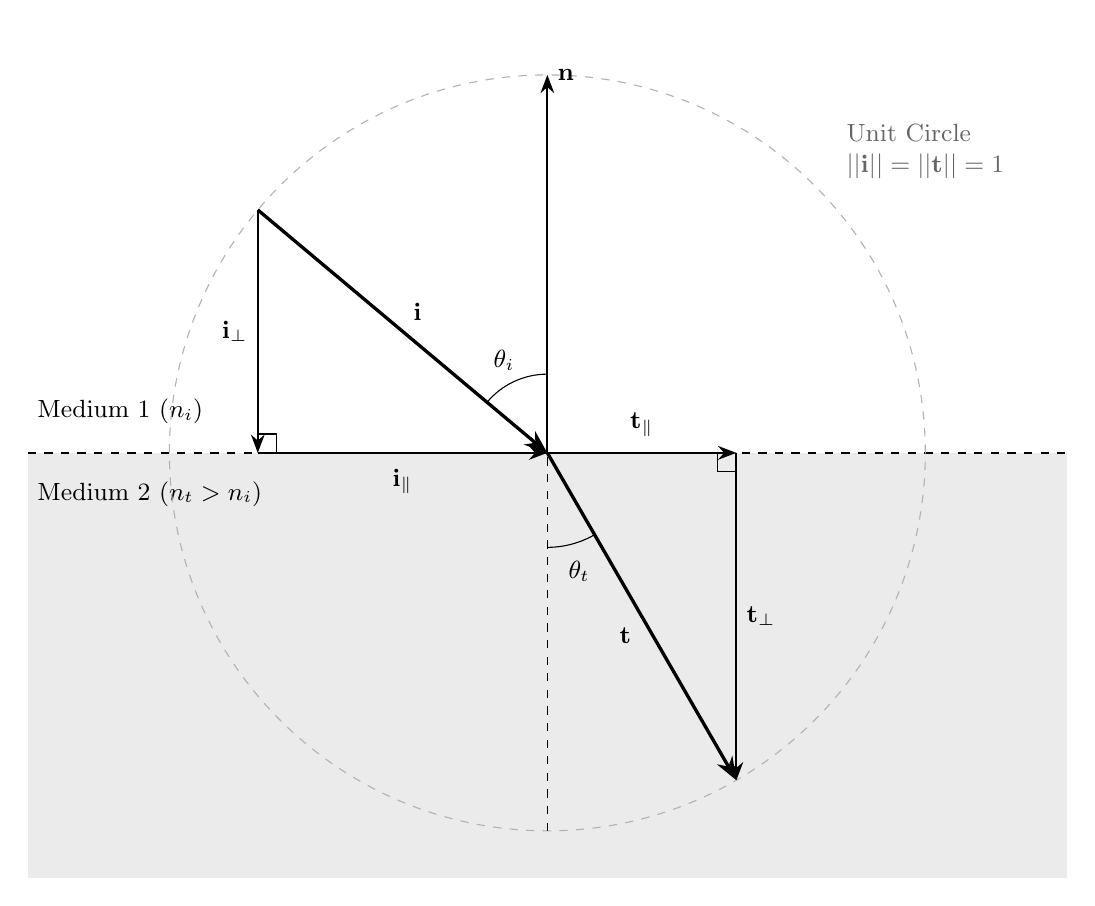
\begin{tikzpicture}[>=Stealth, font=\small, scale=1.2]
    % ================= Parameters =================
    \def\R{4}          % Unit vector radius
    \def\W{5.5}        % Half-width of canvas
    \def\H{4.5}        % Half-height (symmetric about interface y = 0)
    \def\thetaI{50}    % Angle of incidence (degrees)
    \def\thetaT{30}    % Angle of refraction (degrees)

    % Symmetric canvas about the interface
    \path[use as bounding box] (-\W, -\H) rectangle (\W, \H);
    
    % Define key coordinates
    \coordinate (O) at (0,0);
    \coordinate (N_up) at (0, \R);
    \coordinate (N_down) at (0, -\R);
    
    % i and t vectors (Note: i points TO origin, t points FROM origin)
    \coordinate (I) at ({90+\thetaI}:\R);
    \coordinate (T) at ({-90+\thetaT}:\R);
    
    % Projections on the interface
    \coordinate (I_x) at ({-\R*sin(\thetaI)}, 0);
    \coordinate (T_x) at ({\R*sin(\thetaT)}, 0);

    % ================= Background & Interface =================
    % Medium 1 background (white)
    \fill[white] (-\W, 0) rectangle (\W, \H);
    % Medium 2 background (light gray to denote higher index n_t > n_i)
    \fill[black!8] (-\W, -\H) rectangle (\W, 0);

    % Interface line
    \draw[dashed, thick] (-\W, 0) -- (\W, 0);

    % Medium labels (left-aligned at x = -W)
    \node[anchor=south west] at (-\W, 0.2) {Medium 1 ($n_i$)};
    \node[anchor=north west] at (-\W, -0.2) {Medium 2 ($n_t > n_i$)};

    % ================= Unit Circle Auxiliary =================
    \draw[dashed, black!30] (O) circle (\R);
    \node[black!60, above, align=left] at (\R, 2.8) {Unit Circle\\$||\mathbf{i}|| = ||\mathbf{t}|| = 1$};

    % ================= Normal Vector =================
    \draw[dashed] (N_down) -- (O);
    \draw[->, thick] (O) -- (N_up) node[right] {$\mathbf{n}$};

    % ================= Incident Ray & Components =================
    % Components forming vector addition: i_perp + i_parallel = i
    \draw[->, thick] (I) -- (I_x) node[midway, left] {$\mathbf{i}_{\perp}$};
    \draw[->, thick] (I_x) -- (O) node[midway, below=2pt] {$\mathbf{i}_{\parallel}$};
    
    % Right angle symbol for incidence
    \draw (I_x) ++(0.2, 0) -- ++(0, 0.2) -- ++(-0.2, 0);

    % Main incident unit vector
    \draw[->, very thick] (I) -- (O) node[midway, above right] {$\mathbf{i}$};

    % ================= Refracted Ray & Components =================
    % Components forming vector addition: t_parallel + t_perp = t
    \draw[->, thick] (O) -- (T_x) node[midway, above=2pt] {$\mathbf{t}_{\parallel}$};
    \draw[->, thick] (T_x) -- (T) node[midway, right] {$\mathbf{t}_{\perp}$};
    
    % Right angle symbol for refraction
    \draw (T_x) ++(-0.2, 0) -- ++(0, -0.2) -- ++(0.2, 0);

    % Main refracted unit vector
    \draw[->, very thick] (O) -- (T) node[midway, below left] {$\mathbf{t}$};

    % ================= Angles =================
    % Angle of incidence
    \draw pic[draw, angle radius=1cm, "$\theta_i$", angle eccentricity=1.3] {angle = N_up--O--I};
    
    % Angle of refraction
    \draw pic[draw, angle radius=1.2cm, "$\theta_t$", angle eccentricity=1.3] {angle = N_down--O--T};

\end{tikzpicture}
\end{document}